\documentclass{article}
\usepackage[utf8]{inputenc}

\title{Hw1 Report}
\author{Muhammed Yasir Fidan }
\date{April 2021}

\usepackage{natbib}
\usepackage{graphicx}

\begin{document}

\maketitle

\section{Report}
\textbf{Compile and Run} \\
\\
Firstly I compile my program with gcc -o processM hw2.c -std=gnu99 -Wall -D\_BSD\_SOURCE -D\_POSIX\_C\_SOURCE=199309L -lm in makefile, so there is no warning when using -Wall command. After type make and compile program, for running enter ./processM filepath like in homework pdf. filepath is the path of file.
\\
Before running program file look like this. There is a newline at end of row 8 in teacher format file so I write my code according this format. There must be a newline at row 8's end, like in teacher's example file.
\begin{figure}[h!]
\centering
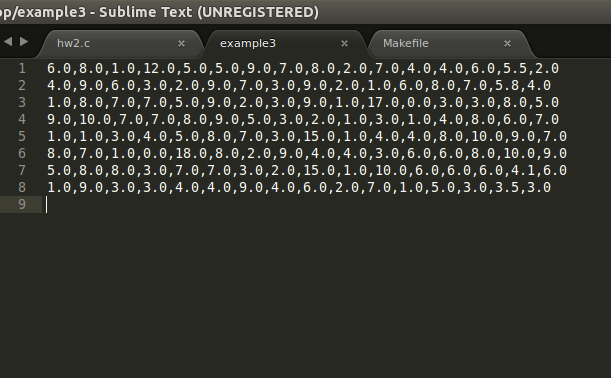
\includegraphics[scale=0.6]{ss1.png}
\caption{File before running}
\label{fig:ss1.png}
\end{figure}

\\
After executing program file will be like this

\begin{figure}[h!]
\centering
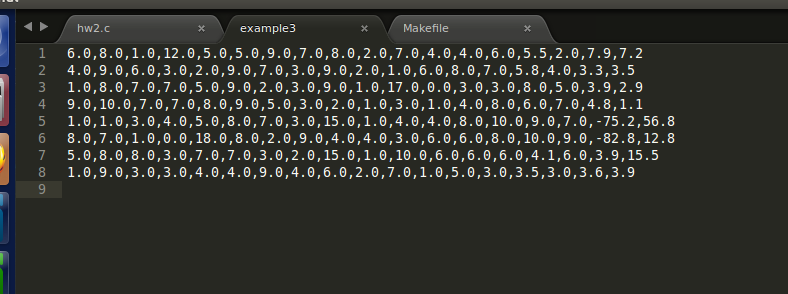
\includegraphics[scale=0.5]{ss2.png}
\caption{File after running}
\label{fig:ss2.png}
\end{figure}
As you can see, after program run each row has 2 more point at the end of the row. New first number is Lagrange of x7 according to first 6 coordinate and second new number at the end of row is Lagrange of x7 according to first 7 coordinate. All row's Lagrange calculated by one child process. For example, first child process calculate first row lagrange for first 6 coordinates and found 7.9 then write it, Then in second round it uses first 7 coordinates and found 7.2 for lagrange of x7 and write it file. Every 8 process calculate and write their results to file like this and so on.

\\
Also After running program, Parent process write error for first round and second round in terminal, Also write each polynomial coefficients.
\\

\begin{figure}[h!]
\centering
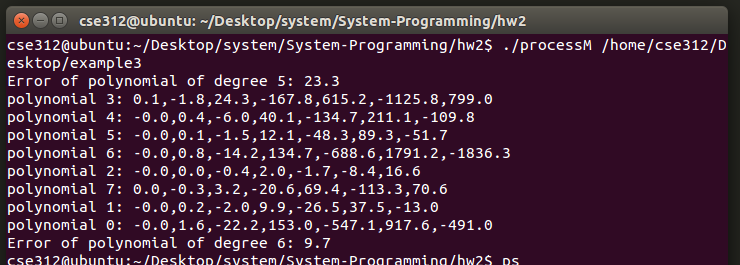
\includegraphics[scale=0.5]{ss3.png}
\caption{Terminal after program run}
\label{fig:ss3.png}
\end{figure}

\newpage
\textbf{
How did I solve file synchronization} \\
\\
There is 8 process that read and write file, So there must be a synchronization for reading and writing. I use fcntl for locking file as suggested in homework pdf, so each child process can read and write file. If there hadn't a file locking system, for example multiple process would read file and change offset or may write at the same time and cause corrupt file. Locking file solve these problems.
\\
\\
\textbf{
How did I solve parent-child synchronization} \\
\\
In this homework, after child write their first calculated value to the file, they must wait and parent must continue, then parent wait and children processes continue. So parent and child must synchronize by using signals. I use only SIGUSR1 signal and sigsuspend for synchronization between parent and child processes. In first part parent use sigsuspend 8 times for waiting SIGUSR1 in his 8 child processes. After child processes calculate their lagrange and write it to the file they send SIGUSR1 by using kill system call to the parent. But there is very tricky problem. What if 2 or more child process send SIGUSR1 signal to parent. In this case because there is no signal pending for more than 1 signal, parent process will execute sigsuspend for only 1 signal, so it lose some children signal and wait infinitely. For solving this problem, I send signal from child before unlocking file and after parent receive signal it send SIGUSR1 to this child to let them know parent receive their signal so they can continue. So with this design parent process can take all 8 signals and then it can continue and children processes once again execute sigsuspend for waiting parent. So all of the children now wait parent to calculate error of degree 5. After parent calcuate error of degree 5 it prints out terminal and send SIGUSR1 all children to make them continue. Now all children process once again continue and calculate new lagrance for their row. After that like in first round, they send signals to parent and wait. After parent continue and print error of polynomial of degree 6 it sends SIGUSR1 to all children to make them continue. Then each child calculate coefficient of each polynomial and print them to screen and terminate.
\\


\begin{figure}[h!]
\centering
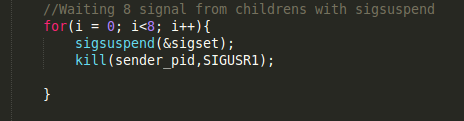
\includegraphics[scale=0.5]{ss4.png}
\caption{Parent wait 8 SIGUSR1 from children}
\label{fig:ss4.png}
\end{figure}
Like above screenshot, Parent process execute 8 sigsuspend to collect all 8 child signal before continue and after it take a signal it send a SIGUSR1 to child process that send SIGUSR1.So if child receive SIGUSR1 it means parent take his signal without any problem.
\begin{figure}[h!]
\centering
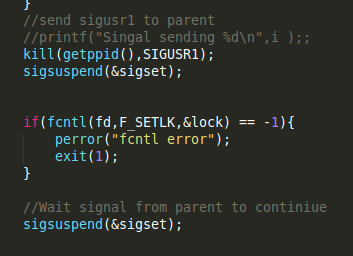
\includegraphics[scale=0.6]{ss5.png}
\caption{Child process send SIGUSR1 to parent}
\label{fig:ss5.png}
\end{figure}

And above screenshot shows that, child process send SIGUSR1 to parent process then suspend for coming signal from parent. After parent send signal it means, parent take his signal without any problem, so child process unlock file and execute sigsuspend once again. So with this design all child process send their signal one by one so parent process can't losing any signal. After parent take all 8 signal it will continue and all child process will be in second sigsuspend for waiting parent.

\begin{figure}[h!]
\centering
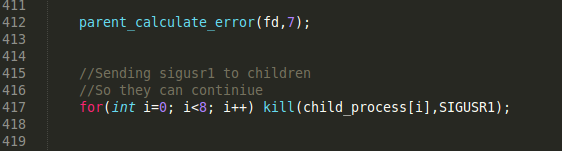
\includegraphics[scale=0.6]{ss6.png}
\caption{Parent calculate error and send signals to children to make them continue}
\label{fig:ss5.png}
\end{figure}
\\
Now parent calculate error for degree 5 and print it to terminal meanwhile all 8 children processes wait parent in sigsuspend. So after parent done it using kill system call to send all 8 children SIGUSR1 signal so know they can continue for second part.
\\ 
Second part again work like this. Again children read and write file for their row's lagrange also they print coefficient of polynomials too. Then parent continue and print error degree of 6.
\newpage
\textbf{
How did I handle zombie process} \\
\\
As mentioned in homework pdf, when a child process terminated a SIGCHLD signal send automatically. So in handler I use wait like we learn in lecture to clean zombie processes.



\begin{figure}[h!]
\centering
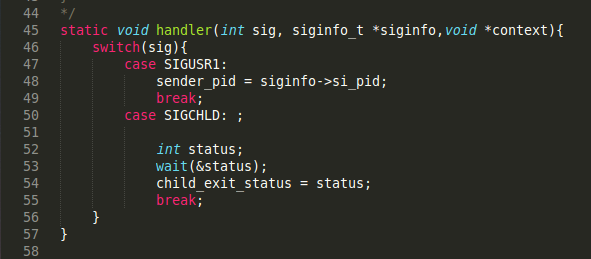
\includegraphics[scale=0.6]{ss7.png}
\caption{Signal handler call wait for SIGCHLD signal}
\label{fig:ss5.png}
\end{figure}

\textbf{
Calculation of polynomial's coefficients} \\
\\
I use gauss elimination method for finding 7 coefficients. Each child process find their corresponding row coefficients by using gauss elimination method. 
\\
\newpage
\textbf{
Valgrind example} \\
When I execute my program with valgrind leak-check=full -v the output like this:

\begin{figure}[h!]
\centering
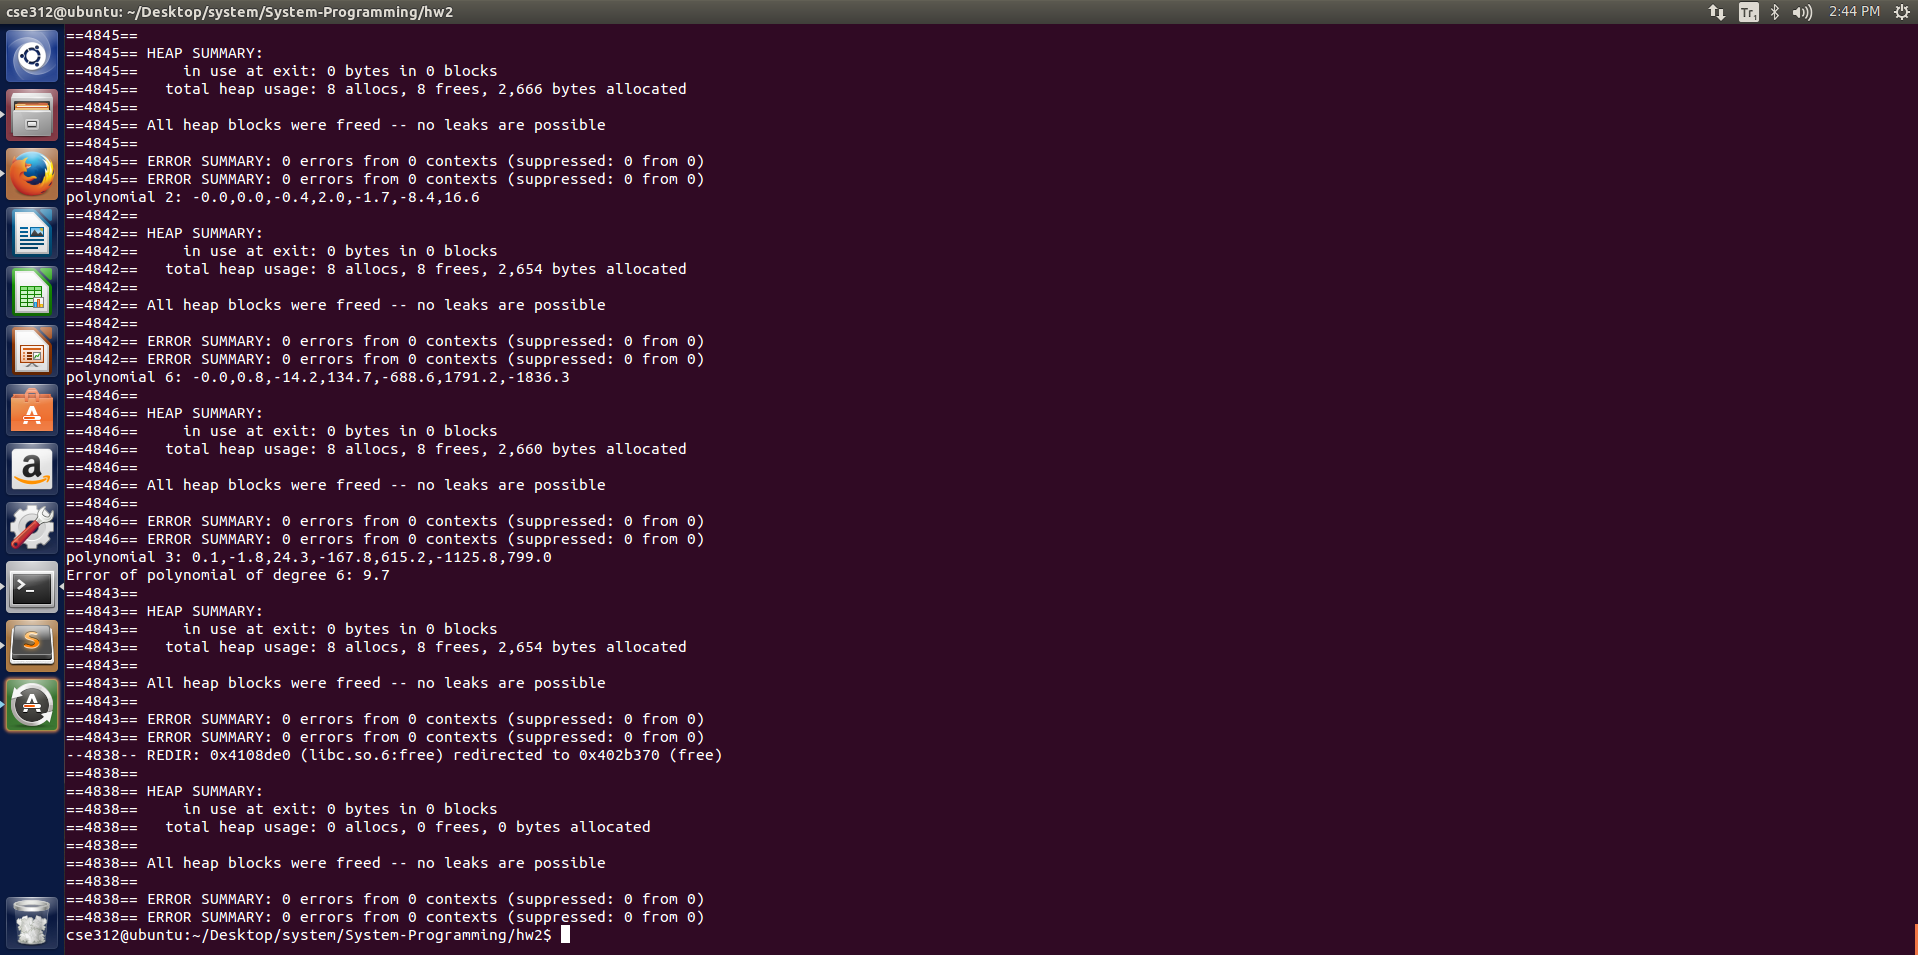
\includegraphics[scale=0.2]{valgrind.png}
\caption{Valgrind leak-ckeck=full -v example}
\label{fig:valgrind.png}
\end{figure}

As you can see there is no leak possible 
\\
\\
Also I only lock files when reading and writing, for example when calculating lagrange formula for both round 1 and round 2 there is no lock so multiple process can calculate their row lagrange at the same time.
\begin{figure}[h!]
\centering
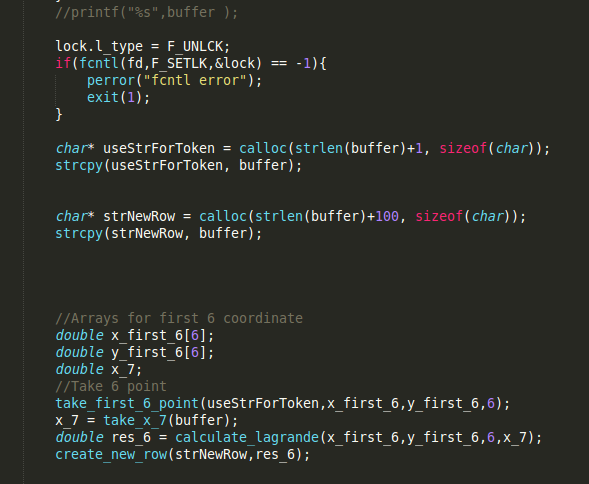
\includegraphics[scale=0.35]{ss8.png}
\caption{No lock when calculating lagrange}
\label{fig:ss8.png}
\end{figure}
\end{document}
